\documentclass[line,margin,colorlinks]{res}
\usepackage[colorlinks=true,urlcolor=cyan]{hyperref}
\usepackage{newcent}
\usepackage[dvipsnames]{xcolor}
\usepackage{tikz}
\usepackage{fontawesome5}
\usepackage[document]{ragged2e}

\begin{document}

\name{Josh Friedlander}
% \address used twice to have two lines of address
\address{\faIcon{home} Epstein 13 Tel Aviv  $\vert$  \faIcon{phone} 0549548448}
\address{\ \ \ \ \ \ \faEnvelope{} \href{mailto:joshuatfriedlander@gmail.com}{joshuatfriedlander@gmail.com}}

\begin{resume}

    \section{SUMMARY}
    \begin{itemize}
        \item I solve business problems with statistical inference and Machine Learning
        \item Technologies: PyData stack \textbf{(Pandas, Numpy, Scikit-Learn, Tensorflow, PyMC3, statsmodels)}, Docker, Kubernetes, the usual cloud providers
        \item Proficient in \textbf{Git, SQL, *nix operating systems}, \{ba,z\}sh scripting
    \end{itemize}


    \rule{13.5cm}{0.4pt}
    \section{WORK \\ EXPERIENCE}
        \textbf{Lead Data Scientist} \\Kando $\vert$ Tzur Yigal, Israel  \hfill \textit{2020-}
    \begin{itemize} \itemsep -2pt % reduce space between items
        \item Developing time-series prediction algorithms for detecting pollution events
        \item Researching anomaly detection and digital signal processing techniques
        \item Writing Python libraries for internal company use (data cleaning, building and parsing tree objects, making Machine Learning models reproducible)
        \item Impromptu data engineer: setting up ML infrastructure and pipeline from ground up, writing Dockerfiles, managing Kubernetes installation
        \item Managing multiple teams of interns, code reviewer for junior developers
    \end{itemize}

        \textbf{Data Scientist} \\Perceptive AI $\vert$ Tel Aviv, Israel  \hfill \textit{2018-2020}
    \begin{itemize}  \itemsep -2pt % reduce space between items
        \item Worked at a seed-stage startup implementing a churn prediction algorithm (Survival Analysis) in the field of Customer Success for SaaS companies
        \item Feature engineering, processing/analysing data, writing algorithms
        \item Wrote scripts in bash and Perl to automate the boring stuff 
        \item Worked in the cloud (AWS), developing on a remote host for data security
        \item Optimised speed and removed bottlenecks within code (e.g.\ by vectorising complex algorithms or researching optimised storage formats)
    \end{itemize}

        \textbf{Data Science Intern} \\Anodot $\vert$ Ra'anana, Israel  \hfill \textit{Fall 2018}
    \begin{itemize}  \itemsep -2pt % reduce space between items
        \item Built LSTM for time-series analysis and compared results with other state-of-the-art methods (e.g. Facebook Prophet)
        \item Worked within production code infrastructure (containers, version control), with emphasis on modular and readable code
    \end{itemize}

    \section{EDUCATION}
      \textbf{Israel Tech Challenge - Data Science Fellow} \hfill \textit{Summer 2018}
    \begin{itemize}  \itemsep -2pt % reduce space between items
        \item Elite ten-month full-time program covering Deep Learning and Computer Vision, emphasising research and self-led learning
        \item Capstone projects: built a web scraper automated with a cron job storing data in a cloud-based DB, and an \href{https://www.itc.tech/an-algorithm-that-predicts-how-funny-a-text-is-yup-its-a-real-thing/}{NLP project} written up for program's blog
    \end{itemize}

      \textbf{B.A. - Jerusalem College of Technology} \hfill {\sl2010-2013}
        % \sl will be bold italic in New Century Schoolbook (or
        % any postscript font) and just slanted in
        % Computer Modern (default) font
    \begin{itemize} \itemsep -2pt
        \item Accounting and Info Systems (probability, stats, databases, SQL, calculus)
        \item Psychometric score: 730
    \end{itemize}

    \section{MISC}
   \textbf{Interests}: \faHiking{} nature walks \faChartLine{} dataviz  \faBiking{} future of mobility \faCoffee{} coffee \faPodcast{} podcasts
      \\ \textbf{Web presence}:
      \raisebox{-4pt}{\begin{tikzpicture} \node[Blue]{\faLinkedin}; \end{tikzpicture}} \href{https://www.linkedin.com/in/josh-friedlander-312b926b}{LinkedIn}
      \raisebox{-4pt}{
\begin{tikzpicture} \node[Orange]{\faIcon{stack-overflow}}; \end{tikzpicture}} \href{https://stackoverflow.com/users/6220759/josh-friedlander}{Stack Overflow}
      \raisebox{-4pt}{\begin{tikzpicture} \node[]{\faGithub}; \end{tikzpicture}} \href{https://github.com/lordgrenville}{GitHub}
      \raisebox{-4pt}{
\begin{tikzpicture} \node[Orange]{\faIcon{hacker-news}}; \end{tikzpicture}} \href{https://news.ycombinator.com/user?id=lordgrenville}{Hacker News}
      \\ \textbf{Languages}: Python, shell, R
      \hspace*{\fill} Hand-written with \raisebox{-4pt}{\begin{tikzpicture} \begin{scope}[] \node[Red]{\faIcon{heart}}; \end{scope} \end{tikzpicture}} in Vim and \LaTeX{}
\end{resume}

\end{document}
